\chapter{Implementation Details}
% This is where you explain what you have implemented and how you have implemented it. Place here all the details that you consider important, organize the chapter in sections and subsections to explain the development and your workflow.\\Given the self-explicative title of the chapter, readers usually skip it. This is ok, because this entire chapter is simply meant to describe the details of your work so that people that are very interested (such as people who have to evaluate your work or people who have to build something more complex starting from what you did) can fully understand what you developed or implemented.\\Don't worry about placing too many details in this chapter, the only essential thing is that you keep everything tidy, without mixing too much information (so make use of sections, subsections, lists, etc.). As usual, pictures are helpful.

\section{Tools used for the Chrome extension}

Extensions are made of different, but cohesive, components. Components can include background scripts, content scripts, an options page, UI elements and various logic files. Extension components are created with web development technologies: HTML, CSS, and JavaScript. An extension's components will depend on its functionality and may not require every option.

In this project the extension was build with the following tools:

\begin{itemize}
    \item HTML
    \item CSS
    \item Typescript
    \item Node
    \item React
    \item Webpack
    \item Material-UI
\end{itemize}

Let's see in the details each of these tools.

\subsection {HTML}

As said in the previous section, the extension is made with the web development technologies. HTML, HyperText Markup Language, is one of them.
In this project, HTML does not have a central role, since it is managed automatically by webpack. However, when the extension is build, the popup and the options main page are in HTML.

\subsection {CSS}

CSS, Cascading Style Sheets, is another web development technology. In this project, CSS is lightly used to style the extension's UI. The majority of the styling part is done through React and Material-UI. However, it's important to mention CSS, since it heavily used and is a key part of the web development workflow.

\subsection {Typescript}

Typescript is a web development technology that is used to write code in a more readable and easy to understand way. In this project, Typescript is used to write the extension's logic.
Typescript is a syntactic superset of Javascript and adds optional static typing to the language. Another difference compared to Javascript is that Typescript is compiled and not interpreted. This means that the extension will not run unless it is compiled. The reason behind the creation of Typescript was the maintenance of large-scale applications. So the decision of using Typescript was made to make the extension's code more maintainable.
In addition, since Typescript has a static typing system, that enables static language analysis, which simplifies the devolopment process by providing meaningful errors.
\subsection {Node}

Node.js is an open-source, cross-platform, back-end JavaScript runtime environment that runs on the V8 engine and executes JavaScript code outside a web browser
Node.js has an event-driven architecture capable of asynchronous I/O. These design choices aim to optimize throughput and scalability in web applications with many input/output operations, as well as for real-time Web applications (e.g., real-time communication programs and browser games).
Node.js allows the creation of Web servers and networking tools using JavaScript and a collection of "modules" that handle various core functionalities.

npm is the pre-installed package manager for the Node.js server platform. It installs Node.js programs from the npm registry, organizing the installation and management of third-party Node.js programs. Packages in the npm registry can range from simple helper libraries to task runners.

\subsection {React}

React (also known as React.js or ReactJS) is a free and open-source front-end JavaScript library for building user interfaces based on UI components. It is maintained by Meta (formerly Facebook) and a community of individual developers and companies. React can be used as a base in the development of single-page, mobile, or server-rendered applications with frameworks like Next.js. However, React is only concerned with state management and rendering that state to the DOM, so creating React applications usually requires the use of additional libraries for routing, as well as certain client-side functionality.

\subsection {Webpack}

Webpack is a free and open-source module bundler for JavaScript. It is made primarily for JavaScript, but it can transform front-end assets such as HTML, CSS, and images if the corresponding loaders are included. Webpack takes modules with dependencies and generates static assets representing those modules.

% insert image
\begin{figure}[h!]
    \vspace{0.5cm}
    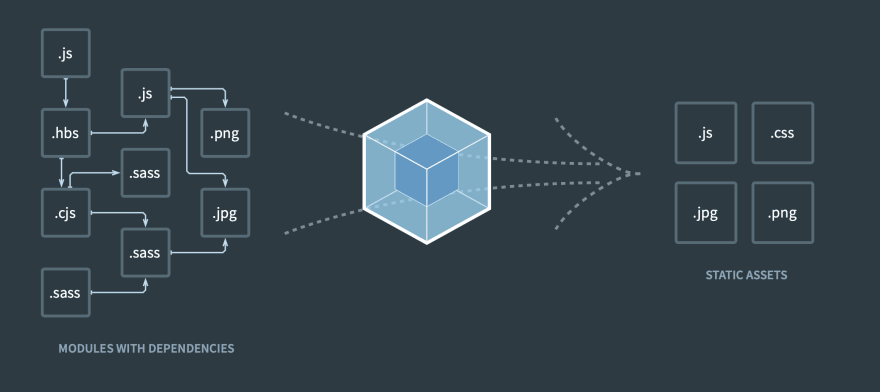
\includegraphics[width=\textwidth]{images/webpack-bundle.png}
    \caption{webpack workflow}
    \label{fig:webpack-bundle} % this is the image label, with which you can refer to the image in any document location.
\end{figure}

\subsection {Material-UI}

Material UI is an open-source React component library that implements Google's Material Design. In this project is used to create the extension's UI.
It includes a comprehensive collection of prebuilt components that are ready for use in production right out of the box.
Material UI is beautiful by design, and features a suite of customization options that make it easy to implement your own custom design system on top of our components.
The main advantages of material UI are:

\begin{itemize}
    \item Ready to use
    \item Follow Google's Material Design so it is consistent with a big part of the web
    \item Realiable with a great community
\end{itemize}


\section {Design Choices}

In this section all design choices are explained. For each key part of the extension there is an image showing it and there is a complete explanation.

\subsection {Popup and Tab Navigation}

The two key elements of the extension are the popup and the tab navigation. The popup is the main window of the extension and the tab navigation is the bottom part of the popup, in which there are the tabs that are used to navigate between the different sections of the extension. The four tabs are:

\begin{enumerate}
    \item \textbf{Tab}: it shows passwords, if there are, for the current website.
    \item \textbf{My Vault}: it shows the passwords that are stored in the vault.
    \item \textbf{Generate}: it allows the user to generate a new password.
    \item \textbf{Add}: it allows the user to add a new password.
\end{enumerate}

% insert image

Another detail in the popup is the lock button. This button, when clicked, blocks the extension. This allows the user to force lock the extension, since the next time it will be opened it will ask for the master password.
The whole popup with the component just described is shown in image \ref*{fig:popup-lock-tab}
% Insert image

% insert image
\begin{figure}[h!]
    \centering
    \vspace{0.5cm}
    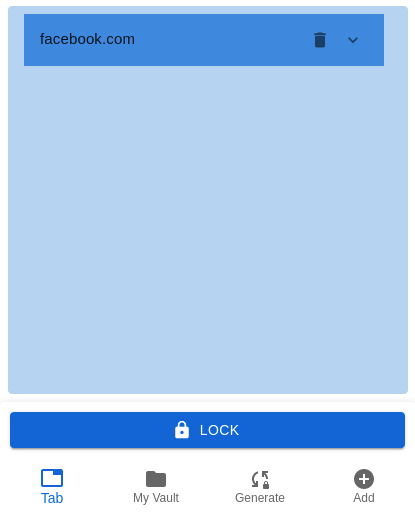
\includegraphics[width=0.5\textwidth]{images/popup-lock-tab.png}
    \caption{Popup, lock button and tabs}
    \label{fig:popup-lock-tab} % this is the image label, with which you can refer to the image in any document location.
\end{figure}

\subsection {Tab}

The tab section of the extension is shown in image \ref{fig:popup-lock-tab}. It's visible that when the user clicks on the extension, the popup opens and the Tab is the default section. In fact, in this section, the user can see the passwords that are stored for the current website.

This is done by retrieving the hostname of the website, and then searching for the website in the vault. If the website is found, the passwords are shown.

\subsection {My Vault}

The My Vault section is shown in image \ref{fig:my-vault}. It's visible that when the user clicks on the extension, the popup opens and the My Vault is the default section. In fact, in this section, the user can see the passwords that are stored in the vault.
% insert image
\begin{figure}[h!]
    \centering
    \vspace{0.5cm}
    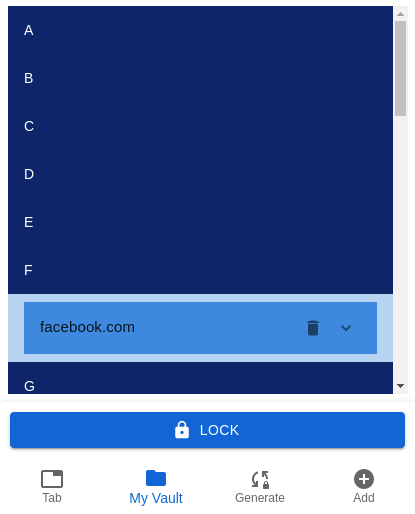
\includegraphics[width=0.5\textwidth]{images/my-vault.png}
    \caption{My Vault section of the extension}
    \label{fig:my-vault} % this is the image label, with which you can refer to the image in any document location.
\end{figure}

\subsubsection{Generate}

% insert image
\begin{figure}[h!]
    \centering
    \vspace{0.5cm}
    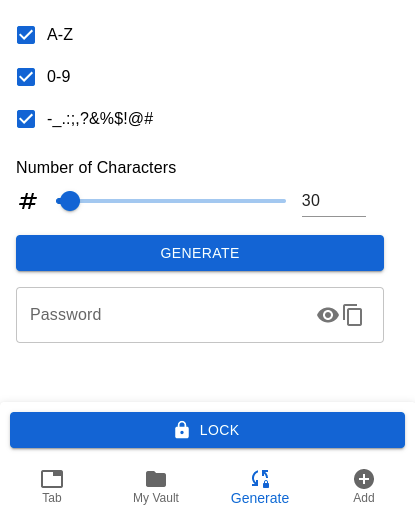
\includegraphics[width=0.5\textwidth]{images/generate.png}
    \caption{Generate section of the extension}
    \label{fig:generate} % this is the image label, with which you can refer to the image in any document location.
\end{figure}

This section is very important, since it is used to generate a new password. The user can choose the length of the password, and the type of characters that will be used. The supported type of characters are:

\begin{itemize}
    \item \textbf{Uppercase}: uppercase letters
    \item \textbf{Numbers}: numbers
    \item \textbf{Special}: special characters
\end{itemize}
If no type of characters is selected, the password will be generated with lowercase letters only.
The generated password is shown in image \ref{fig:generate}

\subsubsection{Add}

The last section of the extension is the Add, that is useful to add a new password to the vault. The logic behind the autocompletion of the hostname is the same as the one from the Tab section.
The Add section is shown in image \ref{fig:add}

% insert image
\begin{figure}[h!]
    \centering
    \vspace{0.5cm}
    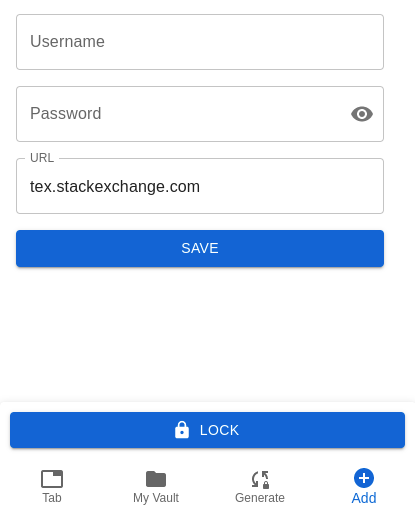
\includegraphics[width=0.5\textwidth]{images/add.png}
    \caption{Add section of the extension}
    \label{fig:add} % this is the image label, with which you can refer to the image in any document location.
\end{figure}


\subsection{Options}

The options are kept as simple as possible. In fact there are only two of them:

\begin{enumerate}
    \item \textbf{Autocomplete}:it allows to autocomplete the login form when the page is uploaded
    \item \textbf{Lock After}: it allows to specify the minutes after which the extension will be locked and ask again the password.
\end{enumerate}

In order to retrieve the options when the users reopens the extension, the local storage is used. Since the options are not sensible data, it is not important that the data are encrypted, and in fact the local storage was the correct choice. In a future implementation, since Chome support by default the sync storage, the options can be stored in the sync storage so that each Chrome browser connected to the same Google account will have the same options. This uses the Google sync API and it can be taken as it is, supposing it is secure out of the box. 

% insert image

\subsection{Expandable Menu and Buttons}

In the section of the extension where we have the entries with the password, there always is a expandable menu. When expanded, the entry shows the username, the password and the URL. The expanded menu is shown in % insert the image

To improve security, the password is hidden by default. This rule applies to all field where there is a password. However, if the user wants to see the password, there is an eye button at the end of the password field, that allows to show the password.

When the menu is expanded, near each field there are two buttons:

\begin{enumerate}
    \item \textbf{Edit}: it allows to edit the field
    \item \textbf{Copy}: it copies the content of the field to the clipboard.
\end{enumerate}

In addition to the expandable menu there is also a button that allows to delete the password. When the button is clicked, the user is prompted with a confirmation dialog. The button of the confirmation dialog are colored in a way such that the delete button is red, and the keep button is green.


\section{Autocomplete}

This feature is a key part of the extension, since it improves drastically the user experience and usability. The extension is able to autocomplete the login form when the page is loaded. 
The idea behind the autocomplete is the following: when the page is loaded, the extension retrieves the username and password text fields. Then, the extension, knowing the current website, makes a request to the Middleware to retrieve the username and password of the website. If the username and password are found, the extension automatically fills the fields. Otherwise, nothing happens.

The autocomplete feature works in conjunction with the lock after. In fact, if the extension is locked, the autocomplete feature is disabled. Indeed, if the extension is unlocked, the autocomplete feature follows what the user set in the options.
\section{Lock After}

This feature is very important from two points of view: first, it allows the user to keep the extension unlocked for a certain period of time avoiding the need to enter the password every time the extension is opened. Second, it allows the user to lock the extension after a certain period of time, and ask again the password. So it touches both usability and security, finding a balance between the two. The is balance stands is the customizability; in fact the time, in minutes, after which the extension will be locked is configurable in the options. 

The implementation is pretty straightforward. When the user unlocks the extension, a timestamp is sent to the Middleware, that saves it. After that, at every request, the Middleware checks if the current timestamp is greater than the saved timestamp. If it is, the Middleware returns 403, and so the extension is locked. Otherwise, the Middleware returns the asked data. 
